\documentclass[12pt,a4paper]{article}
\usepackage[T1]{fontenc}
\usepackage[utf8]{inputenc}
\usepackage[spanish,es-tabla]{babel}
\usepackage{lmodern,microtype}
\usepackage[a4paper,top=2.5cm,bottom=2.35cm,left=2.45cm,right=2.45cm]{geometry}
\usepackage{graphicx}
\usepackage{longtable,booktabs,array}
\usepackage{enumitem}
\usepackage{csquotes}
\usepackage[hidelinks]{hyperref}
\usepackage[backend=biber,style=ieee,sorting=none]{biblatex}
\addbibresource{referencias.bib}
\setlength{\parindent}{0.9cm}
\setlength{\parskip}{3pt}
\setlength{\tabcolsep}{4pt}
\renewcommand{\arraystretch}{1.16}
\newcolumntype{P}[1]{>{\raggedright\arraybackslash}p{#1}}
\setlist[enumerate]{leftmargin=*,itemsep=4pt}
\begin{document}
\begin{titlepage}
\begin{center}
{\Large\bfseries Universidad Técnica Estatal de Quevedo}\\[0.4cm]
{\bfseries Facultad de Ciencias de la Computación}\\[0.2cm]
{\bfseries Carrera de Software}\\[0.85cm]
{\Large Ingeniería de Requisitos (ISR-401)}\\[1.3cm]
{\LARGE\bfseries TA-TAR-01 --- SUM}\\[0.45cm]
{\Large\bfseries IEEE 29148 y tipos de requisitos de un sistema conocido}\\[0.8cm]
{\large\bfseries Mi Claro Ecuador: portal móvil Activa Claro}\\[1.35cm]
\end{center}
\noindent\textbf{Estudiante:} Cristopher Lavayen\\[0.2cm]
\textbf{Modalidad:} Individual\\[0.2cm]
\textbf{Periodo académico:} SPA 2026--2027\\[0.2cm]
\textbf{Fecha límite original:} 7 de noviembre de 2026
\vfill
\begin{center}Quevedo, Ecuador\end{center}
\end{titlepage}
\section{Resumen analítico: redactar requisitos que sirvan}

\textbf{Primero hay que entender el problema.} Cuando una persona busca un paquete de internet para su celular, no empieza pensando en documentos técnicos: mira cuánto cuesta, cuántos gigabytes incluye y hasta cuándo puede usarlo. En una misma pantalla pueden aparecer ofertas de uno, tres o quince días. Esas diferencias parecen obvias, pero si un sistema no las presenta correctamente, el cliente puede tomar una decisión equivocada. Al analizar el portal Activa Claro, esa situación permite entender por qué los requisitos deben escribirse con detalle.

La norma ISO/IEC/IEEE 29148:2018 establece un marco para recopilar, organizar y revisar requisitos a lo largo del trabajo con sistemas y software. Su definición del apartado \textbf{3.1.19} señala que un requisito expresa una necesidad junto con sus límites y condiciones relacionadas \cite{ieee29148}. Por ejemplo, pedir ``mostrar paquetes'' es apenas una idea inicial. Para convertirla en algo útil hay que indicar qué paquetes, qué información se presenta y cómo se reconoce que la pantalla respondió correctamente.

\textbf{De la petición a una decisión de diseño.} El apartado \textbf{5.2.3} trata la transformación de necesidades en requisitos. Esa transformación requiere entender las tareas reales de las personas antes de decidir cómo resolverlas. Las capturas de este estudio dejan ver botones para comprar paquetes, recargar saldo, regalar paquetes y consultar el historial de compras. No obstante, ver un botón no demuestra que el servicio siempre funcione ni que una compra se complete correctamente. Es una evidencia de interfaz, no de todos los procesos que ocurren por detrás.

En una investigación real sería necesario preguntar a quienes utilizan estas opciones qué dificultades encuentran. Una persona podría querer ordenar paquetes por tiempo de duración porque solo necesita internet para un fin de semana. Otra quizá necesita comprobar el precio final antes de aceptar una compra. Las dos situaciones se relacionan con el catálogo, pero conducen a requisitos distintos. La norma ayuda a evitar que se mezclen decisiones sin haber aclarado antes la necesidad.

\textbf{Qué hace que un requisito esté bien escrito.} En el apartado \textbf{5.2.4}, ISO/IEC/IEEE 29148 describe la construcción de requisitos bien formulados. El enunciado debe referirse a una capacidad, una propiedad o una condición del sistema, delimitar su alcance y permitir una comprobación. Es diferente escribir ``el portal debe ser cómodo'' y especificar que un usuario podrá filtrar paquetes por su vigencia y reconocer la categoría que ha seleccionado. La segunda frase describe una acción observable.

Un requisito también tiene que evitar imponer elementos que no sean necesarios. Si lo importante es comparar paquetes, pedir directamente una tecnología de programación concreta puede distraer del objetivo, salvo que exista una restricción que lo justifique. Tampoco es adecuado reunir varias acciones independientes en una sola frase. Consultar un paquete, confirmar un pago y mostrar su historial pueden estar conectados, pero cada operación necesita su propio criterio de aceptación.

\textbf{Revisar cada enunciado.} El apartado \textbf{5.2.5} presenta nueve propiedades para examinar un requisito individual. Debe ser necesario y apropiado para el nivel que se está describiendo; no ambiguo, completo y singular; posible de realizar y verificar; correcto respecto a la necesidad original; y conforme con la forma de documentación que se haya establecido \cite{ieee29148}. Si se escribe que ``la página abrirá rápido'', falta información para evaluar el resultado. Nadie sabría si dos, cinco o diez segundos son aceptables.

También hay que cuidar las palabras de uso cotidiano. Expresiones como ``sin errores'', ``muy fácil'', ``instantáneo'' o ``seguro'' suelen entenderse de varias maneras. La norma no consiste en prohibir vocablos de una lista: lo importante es que el requisito tenga una interpretación clara. En el caso del catálogo de Claro, medir el tiempo que tarda en aparecer una lista de ofertas puede ser más útil que utilizar un adjetivo. El límite elegido, además, debe discutirse con los interesados; no se vuelve una exigencia oficial solamente porque se escriba en el informe.

\textbf{Mirar el conjunto completo.} El apartado \textbf{5.2.6} se ocupa de las propiedades del grupo de requisitos. No basta con que cada frase sea comprensible por separado. También es necesario comprobar que no existan contradicciones, omisiones o condiciones imposibles de aplicar simultáneamente. Si el catálogo promete un paquete de tres días y el resumen de compra indica uno, el problema aparece aunque cada pantalla parezca ordenada. Lo mismo ocurriría si la página permite cambiar de línea, pero el historial muestra operaciones de otra persona.

Analizar los requisitos como conjunto permite relacionar el menú, los filtros, las ofertas y las compras. También ayuda a distinguir las funciones visibles de las condiciones de seguridad y disponibilidad, que requieren otro tipo de pruebas. ISO/IEC 25010:2023 proporciona categorías para describir la calidad del producto, como eficiencia del desempeño, fiabilidad, seguridad y capacidad de interacción \cite{iso25010}. Aquí se usan esas categorías para plantear objetivos medibles, sin afirmar que Claro ya haya sido evaluado bajo esos valores.

El ejercicio deja una idea práctica: redactar requisitos significa convertir situaciones concretas en compromisos claros. Una observación en pantalla sirve para plantear preguntas; una especificación adecuada sirve para acordar qué se hará; y una prueba permite comprobar más adelante si se consiguió. Confundir esas etapas llevaría a conclusiones que las tres capturas no pueden respaldar.

Hay además dos preguntas diferentes: si el requisito está bien redactado y si realmente representa lo que necesita la persona. La primera se estudia mediante la verificación de requisitos; la segunda, mediante la validación con interesados. En el caso de Claro, un requisito puede indicar de forma precisa que las tarjetas muestren precio, beneficio y vigencia. Sería posible revisar si ese texto está completo. Sin embargo, todavía faltaría preguntar a los usuarios si esos tres datos son suficientes para escoger un paquete. Quizás también necesitan saber qué ocurre con el saldo cuando vence la promoción.

Esta distinción es importante para no evaluar un sistema únicamente por lo que se ve. Un menú puede tener buena presentación y aun así carecer de información esencial. Del mismo modo, una regla que parece correcta puede fallar cuando se aplica a un número equivocado o a una oferta que ya terminó. Antes de aceptar el conjunto de requisitos habría que revisar esos casos con ejemplos de compra, recarga y consulta. Así las pruebas posteriores responderían a necesidades reales, no solo a la apariencia de la página.
\clearpage
\section{Diez conceptos de la cláusula 3}
Las explicaciones son paráfrasis sencillas de términos recogidos en la cláusula 3 de ISO/IEC/IEEE 29148:2018 \cite{ieee29148}.
\begin{enumerate}
\item \textbf{Adquirente (3.1.1).} Quien consigue un producto o contrata un servicio. \emph{Ejemplo:} una persona que compra un paquete de internet móvil.
\item \textbf{Atributo (3.1.2).} Propiedad que se puede describir o medir. \emph{Ejemplo:} la duración de un paquete, expresada en días.
\item \textbf{Línea base (3.1.3).} Versión aprobada que se conserva como referencia para controlar cambios. \emph{Ejemplo:} la lista de requisitos aceptada antes de modificar el menú de compras.
\item \textbf{Especificación de requisitos del negocio (3.1.4).} Documento que reúne lo que una organización necesita conseguir y sus límites. \emph{Ejemplo:} describir las condiciones generales que debe respetar la venta digital de paquetes.
\item \textbf{Concepto de operaciones (3.1.5).} Explicación general de cómo se espera que una organización lleve a cabo sus actividades. \emph{Ejemplo:} un esquema que muestre la compra de paquetes desde la elección hasta la confirmación.
\item \textbf{Condición (3.1.6).} Circunstancia en la que se aplica un requisito. \emph{Ejemplo:} mostrar los datos del paquete antes de aceptar el pago.
\item \textbf{Restricción (3.1.7).} Límite que el sistema o su desarrollo no puede ignorar. \emph{Ejemplo:} cumplir la legislación sobre datos personales.
\item \textbf{Contexto de uso (3.1.8).} Personas, tareas y entorno en los que se utiliza el producto. \emph{Ejemplo:} consultar ofertas desde un celular usando una conexión móvil.
\item \textbf{Cliente (3.1.9).} Persona u organización que recibe o puede recibir el servicio. \emph{Ejemplo:} el titular de una línea prepago que solicita una recarga.
\item \textbf{Requisito derivado (3.1.10).} Necesidad que surge al ordenar y desarrollar otros requisitos. \emph{Ejemplo:} guardar la categoría seleccionada cuando se exige que una consulta continúe después de un corte de conexión.
\end{enumerate}
\section{Caso analizado y evidencias}
El tema elegido es el portal móvil de Claro Ecuador que se abre desde un navegador en \texttt{activa.claro.com.ec}. En este informe se lo relaciona con la autogestión de Mi Claro, pero no se presenta como si las capturas provinieran de la aplicación nativa. La propia empresa ofrece canales digitales para adquirir paquetes y realizar recargas \cite{claroRecargas}.

En la primera captura se observan paquetes destacados y accesos para contratar servicios. La segunda muestra el catálogo, con categorías como Vigencia, Minutos y Redes. La tercera enseña el menú completo, que incluye recargas, suscripciones, regalos, historial de compras y tarjetas. Las imágenes son material aportado por el estudiante; el número de teléfono se ocultó antes de incorporarlas al informe.
\begin{figure}[p]
\centering
\begin{minipage}[t]{0.49\textwidth}
\centering
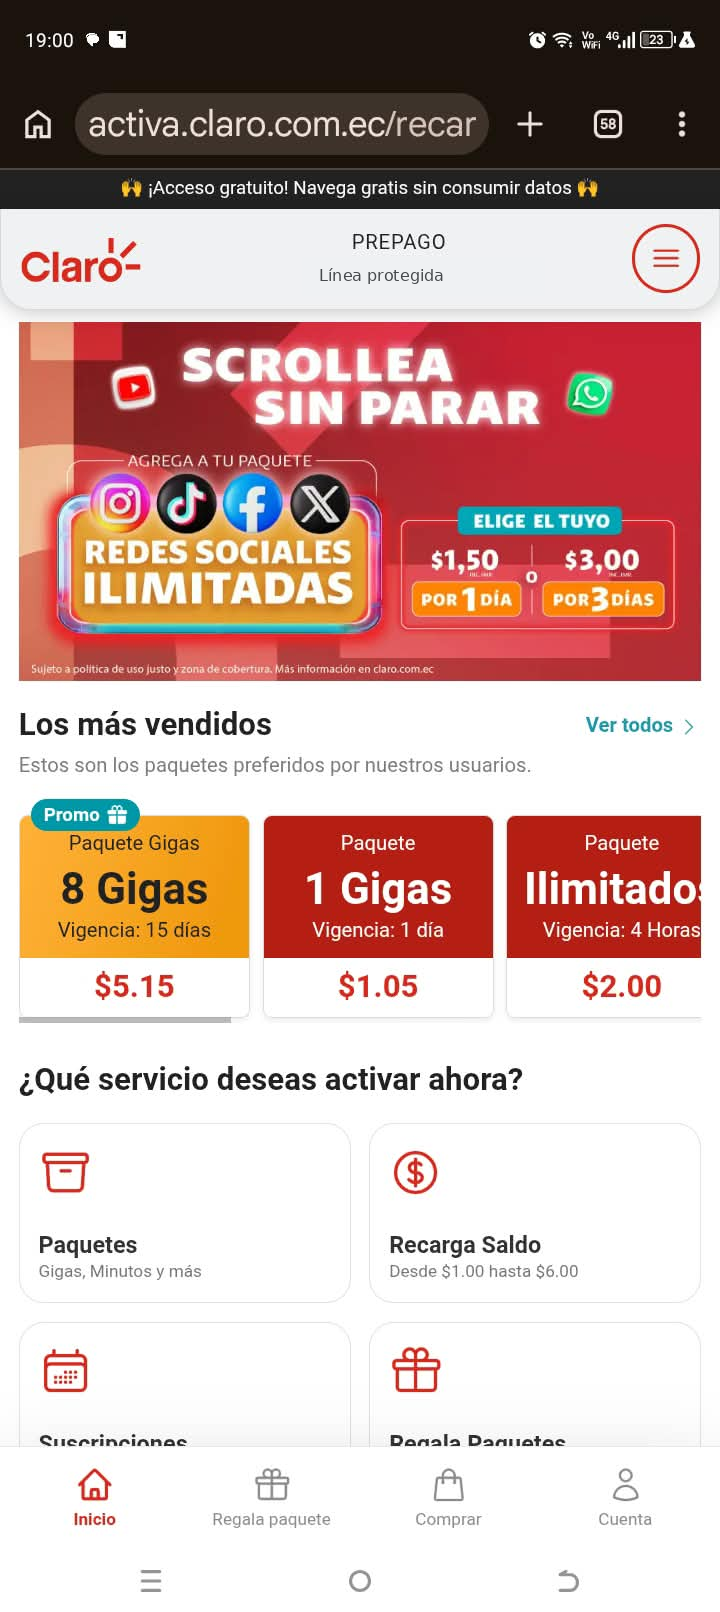
\includegraphics[height=12.8cm,keepaspectratio]{evidencias/captura1.png}
\caption{Inicio del portal, con ofertas y accesos a servicios.}
\end{minipage}\hfill
\begin{minipage}[t]{0.49\textwidth}
\centering
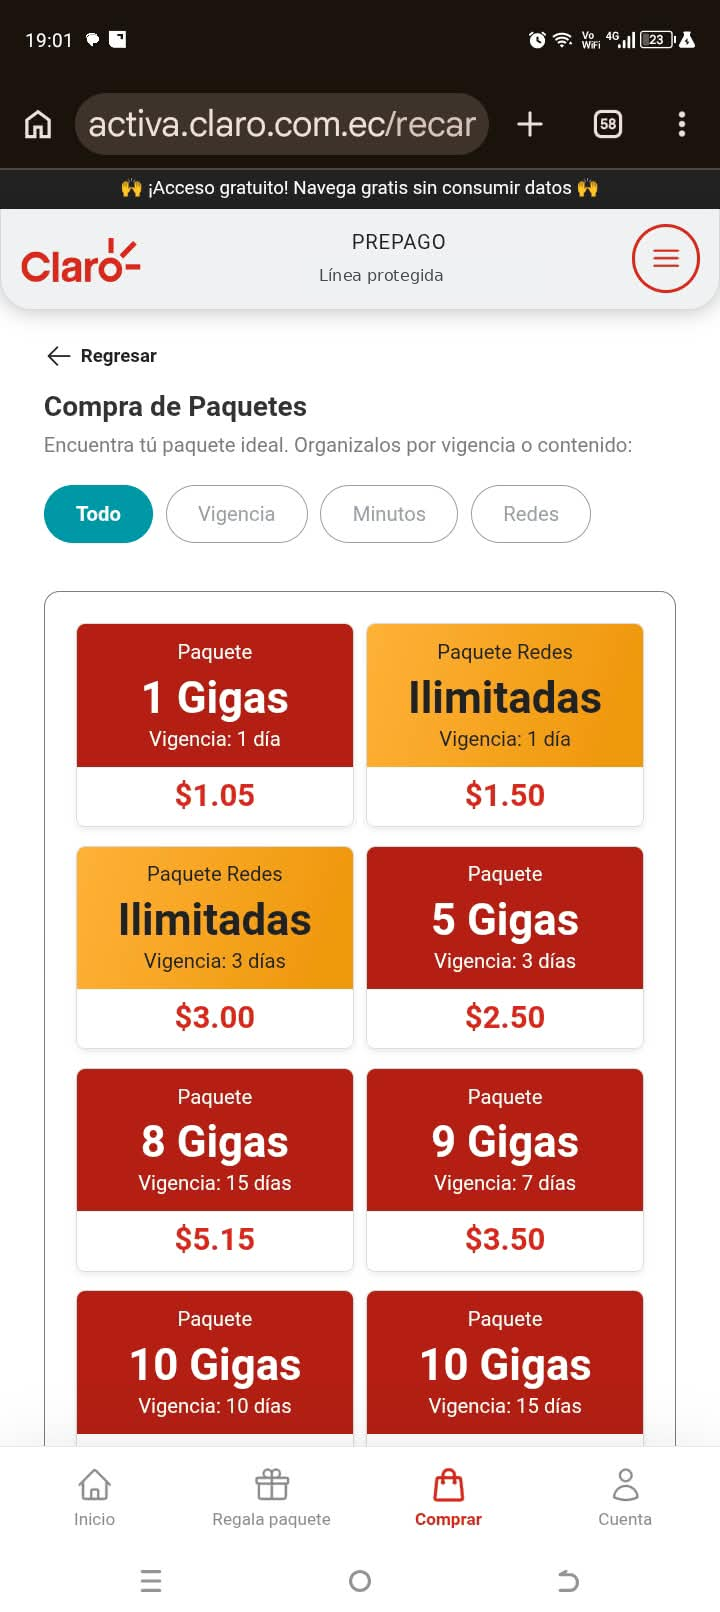
\includegraphics[height=12.8cm,keepaspectratio]{evidencias/captura2.png}
\caption{Paquetes disponibles, filtros, precio y vigencia.}
\end{minipage}
\end{figure}
\begin{figure}[p]
\centering
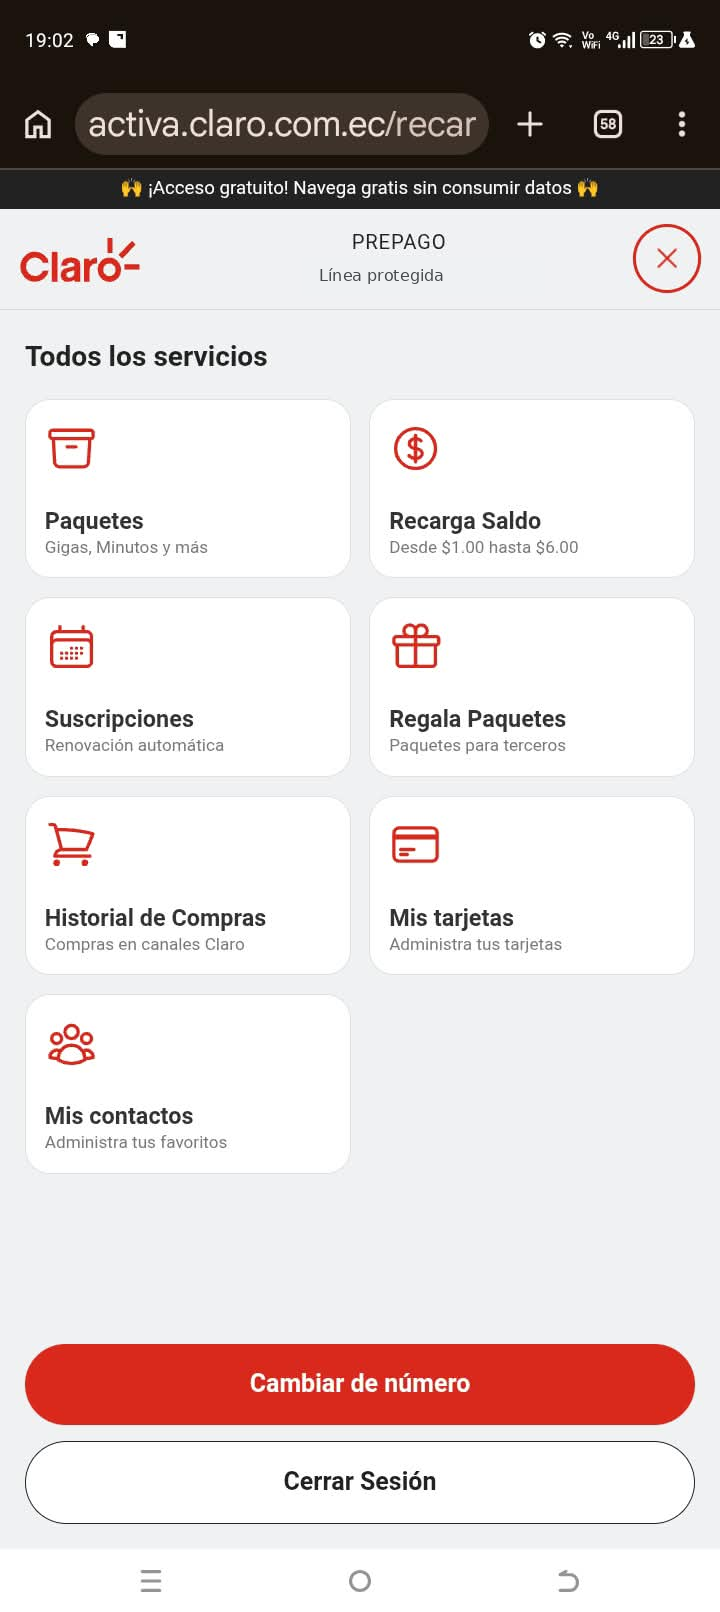
\includegraphics[height=13.5cm,keepaspectratio]{evidencias/captura3.png}
\caption{Menú completo de opciones de autogestión.}
\end{figure}
\clearpage
\section{Quince requisitos propuestos}
Se establecen cinco grupos para separar acciones, atributos de calidad, elementos de pantalla, reglas del negocio y restricciones. Los tiempos y porcentajes de esta sección son \emph{objetivos propuestos para el ejercicio}; no son estadísticas publicadas por Claro ni resultados de una prueba realizada.

\subsection{Funciones del portal (4)}

\noindent\textbf{RF-01: Elegir un tipo de paquete.} El portal deberá permitir que el visitante consulte paquetes desde las categorías Vigencia, Minutos y Redes, además de la vista general.


\noindent\textbf{RF-02: Consultar una oferta.} El portal deberá abrir el detalle del paquete elegido con su contenido, precio en dólares y días u horas de vigencia antes de iniciar una compra.


\noindent\textbf{RF-03: Acceso a recargas.} La sección de servicios deberá ofrecer una opción llamada Recarga Saldo que conduzca al proceso de recarga de la línea seleccionada.


\noindent\textbf{RF-04: Abrir el historial.} Cuando el titular escoja Historial de Compras, el portal deberá mostrar las transacciones asociadas a la línea activa, ordenadas de la más reciente a la más antigua.


\subsection{Características de calidad (5)}

\noindent\textbf{RC-01: Carga del catálogo.} Durante cien aperturas del catálogo con conexión móvil estable, al menos noventa y cinco deberán completar la carga en un máximo de tres segundos.


\noindent\textbf{RC-02: Uso de filtros.} En una prueba con veinte personas que usan por primera vez el portal, al menos dieciocho deberán encontrar un paquete de tres días mediante los filtros en menos de dos minutos y sin recibir instrucciones.


\noindent\textbf{RC-03: Privacidad de la línea.} En una prueba con cincuenta peticiones de una cuenta sin permiso sobre el historial de otra línea, el portal deberá bloquear las cincuenta sin revelar datos de compras.


\noindent\textbf{RC-04: Acceso al servicio.} El catálogo de paquetes deberá estar disponible al menos el 99,5\% del tiempo durante una medición de treinta días seguidos.


\noindent\textbf{RC-05: Continuidad de navegación.} Si la conexión se interrumpe por veinte segundos mientras se consulta el catálogo, el portal deberá recuperar la categoría seleccionada en veinte segundos o menos después de volver a disponer de internet en al menos diecinueve de veinte intentos.


\subsection{Presentación e interfaz (2)}

\noindent\textbf{RI-01: Tarjetas comparables.} Cada tarjeta del catálogo deberá presentar el nombre o beneficio del paquete, el precio en USD y el periodo de validez con sus unidades visibles.


\noindent\textbf{RI-02: Menú de servicios.} Al abrir Todos los servicios, la pantalla deberá mostrar opciones identificables de Paquetes, Recarga Saldo, Suscripciones, Regala Paquetes e Historial de Compras.


\subsection{Reglas de negocio (2)}

\noindent\textbf{RN-01: Duración ofrecida.} Para cada paquete confirmado, la vigencia que se registre deberá ser igual a la duración que el usuario vio en la oferta seleccionada antes de pagar.


\noindent\textbf{RN-02: Importe aceptado.} Una compra de paquete deberá mostrar para confirmación el mismo precio final que figuraba en la oferta elegida, salvo que se informe explícitamente un cambio antes de pagar.


\subsection{Restricciones (2)}

\noindent\textbf{RT-01: Uso desde navegador móvil.} La solución considerada deberá permitir consultar paquetes y abrir el menú desde un navegador móvil a partir de 360 píxeles de ancho, sin desplazamiento lateral para esas tareas.


\noindent\textbf{RT-02: Protección de datos personales.} El tratamiento de números telefónicos y datos de compra deberá ajustarse a las obligaciones aplicables de la Ley Orgánica de Protección de Datos Personales del Ecuador \cite{leyDatos}.

\subsection{Métricas de los requisitos de calidad}
Las cinco condiciones de calidad se relacionan con ISO/IEC 25010:2023 \cite{iso25010}. Esta tabla precisa la medida, la unidad y el límite que permitirían revisarlas.
\small
\begin{longtable}{@{}P{1.25cm}P{4.4cm}P{3.2cm}P{4.75cm}@{}}
\toprule
\textbf{ID} & \textbf{Característica / subcaracterística} & \textbf{Métrica y unidad} & \textbf{Umbral propuesto}\\\midrule
\endfirsthead
\toprule\textbf{ID} & \textbf{Característica / subcaracterística} & \textbf{Métrica y unidad} & \textbf{Umbral propuesto}\\\midrule
\endhead
RC-01 & Eficiencia del desempeño / comportamiento temporal & Tiempo de carga, segundos & Al menos 95 de 100 cargas en 3 s o menos.\\
RC-02 & Capacidad de interacción / operabilidad & Tareas completadas y segundos & Al menos 18 de 20 usuarios en menos de 120 s.\\
RC-03 & Seguridad / confidencialidad & Solicitudes denegadas, porcentaje & 50 de 50 solicitudes sin permiso rechazadas.\\
RC-04 & Fiabilidad / disponibilidad & Tiempo de servicio, porcentaje & Disponibilidad mensual mínima del 99,5\\%.\\
RC-05 & Fiabilidad / recuperabilidad & Reanudaciones y segundos & 19 de 20 consultas recuperadas en 20 s o menos.\\
\bottomrule
\end{longtable}
\normalsize
\section{Clasificación y criterios de aceptación}
Cada criterio representa una comprobación que podría ejecutarse en un entorno de pruebas autorizado. No se declara que estas pruebas ya se hayan hecho.
\small
\begin{longtable}{@{}P{1.30cm}P{3.35cm}P{9.05cm}@{}}
\toprule
\textbf{ID} & \textbf{Tipo} & \textbf{Criterio de aceptación}\\\midrule
\endfirsthead
\toprule\textbf{ID} & \textbf{Tipo} & \textbf{Criterio de aceptación}\\\midrule
\endhead
RF-01 & Funcional & Al elegir cada categoría, aparecen paquetes asociados a la categoría seleccionada y queda visible el filtro activo.\\
RF-02 & Funcional & Al seleccionar un paquete de prueba, se presenta su cantidad o beneficio, el importe y la duración de la oferta.\\
RF-03 & Funcional & Desde Todos los servicios, la opción Recarga Saldo abre la pantalla de recarga sin cambiar la línea activa.\\
RF-04 & Funcional & Con una cuenta de prueba que tenga dos compras registradas, solo aparecen las de su línea y se ordenan por fecha descendente.\\
RC-01 & Calidad: desempeño & En 100 mediciones, por lo menos 95 duran 3 segundos o menos desde que se abre el catálogo hasta que se ven las tarjetas.\\
RC-02 & Calidad: interacción & Como mínimo 18 participantes de 20 completan la búsqueda usando el filtro en menos de 120 segundos.\\
RC-03 & Calidad: seguridad & Se deniegan 50 de 50 peticiones no autorizadas y ninguna devuelve contenido de otro titular.\\
RC-04 & Calidad: fiabilidad & Un registro continuo de 30 días confirma disponibilidad mayor o igual al 99,5\%.\\
RC-05 & Calidad: fiabilidad & En 19 de 20 pruebas se conserva la categoría escogida y puede retomarse la consulta antes de 20 segundos desde la reconexión.\\
RI-01 & Interfaz & En una muestra de 10 tarjetas se distinguen beneficio, importe en USD y duración con días u horas.\\
RI-02 & Interfaz & El menú despliega las cinco opciones con textos legibles y permite seleccionarlas por separado.\\
RN-01 & Regla de negocio & En diez compras simuladas, la duración mostrada antes de confirmar coincide con la registrada para las diez activaciones.\\
RN-02 & Regla de negocio & En diez transacciones simuladas el total coincide con el precio anunciado o informa el cambio antes de solicitar confirmación.\\
RT-01 & Restricción técnica & En una ventana de 360 px se usan el menú y el catálogo sin desplazamiento horizontal.\\
RT-02 & Restricción legal & Una revisión legal y técnica documenta las bases de tratamiento, medidas de protección y derechos del titular aplicables a esos datos.\\
\bottomrule
\end{longtable}
\normalsize
\section{Autoevaluación de los quince requisitos}
En cada caso se compara una frase inicial poco útil con una formulación que indica mejor el comportamiento o la condición esperada. La revisión utiliza como referencia las propiedades del apartado 5.2.5 de IEEE 29148:2018 \cite{ieee29148}.
\begin{enumerate}[leftmargin=*,itemsep=7pt]

\item \textbf{RF-01.} \textbf{Primera frase:} Se deben mostrar paquetes por tipo. \textbf{Problema:} La frase no explica qué tipos existen ni cómo se seleccionan. \textbf{Versión corregida:} El portal deberá permitir que el visitante consulte paquetes desde las categorías Vigencia, Minutos y Redes, además de la vista general.

\item \textbf{RF-02.} \textbf{Primera frase:} Permitir ver las ofertas. \textbf{Problema:} No especifica los datos que el visitante necesita para decidir. \textbf{Versión corregida:} El portal deberá abrir el detalle del paquete elegido con su contenido, precio en dólares y días u horas de vigencia antes de iniciar una compra.

\item \textbf{RF-03.} \textbf{Primera frase:} Debe haber recargas. \textbf{Problema:} No describe la acción del usuario ni el resultado esperado. \textbf{Versión corregida:} La sección de servicios deberá ofrecer una opción llamada Recarga Saldo que conduzca al proceso de recarga de la línea seleccionada.

\item \textbf{RF-04.} \textbf{Primera frase:} Tener historial. \textbf{Problema:} Falta indicar de qué compras se trata y el orden de presentación. \textbf{Versión corregida:} Cuando el titular escoja Historial de Compras, el portal deberá mostrar las transacciones asociadas a la línea activa, ordenadas de la más reciente a la más antigua.

\item \textbf{RC-01.} \textbf{Primera frase:} La lista de paquetes cargará veloz. \textbf{Problema:} Veloz no ofrece una medida de tiempo. \textbf{Versión corregida:} Durante cien aperturas del catálogo con conexión móvil estable, al menos noventa y cinco deberán completar la carga en un máximo de tres segundos.

\item \textbf{RC-02.} \textbf{Primera frase:} El catálogo será muy simple. \textbf{Problema:} No se sabe para quién ni qué acción debe resultar sencilla. \textbf{Versión corregida:} En una prueba con veinte personas que usan por primera vez el portal, al menos dieciocho deberán encontrar un paquete de tres días mediante los filtros en menos de dos minutos y sin recibir instrucciones.

\item \textbf{RC-03.} \textbf{Primera frase:} Las compras estarán protegidas. \textbf{Problema:} No se indica frente a qué acceso hay que proteger los datos. \textbf{Versión corregida:} En una prueba con cincuenta peticiones de una cuenta sin permiso sobre el historial de otra línea, el portal deberá bloquear las cincuenta sin revelar datos de compras.

\item \textbf{RC-04.} \textbf{Primera frase:} El portal funcionará todo el tiempo. \textbf{Problema:} Todo el tiempo no define una medición realista. \textbf{Versión corregida:} El catálogo de paquetes deberá estar disponible al menos el 99,5\% del tiempo durante una medición de treinta días seguidos.

\item \textbf{RC-05.} \textbf{Primera frase:} El portal se recuperará sin problema. \textbf{Problema:} No describe el corte de red ni el tiempo máximo de recuperación. \textbf{Versión corregida:} Si la conexión se interrumpe por veinte segundos mientras se consulta el catálogo, el portal deberá recuperar la categoría seleccionada en veinte segundos o menos después de volver a disponer de internet en al menos diecinueve de veinte intentos.

\item \textbf{RI-01.} \textbf{Primera frase:} Las tarjetas tendrán información. \textbf{Problema:} No indica cuáles son los datos importantes ni sus unidades. \textbf{Versión corregida:} Cada tarjeta del catálogo deberá presentar el nombre o beneficio del paquete, el precio en USD y el periodo de validez con sus unidades visibles.

\item \textbf{RI-02.} \textbf{Primera frase:} El menú será claro. \textbf{Problema:} Claro admite interpretaciones distintas y no enumera las opciones. \textbf{Versión corregida:} Al abrir Todos los servicios, la pantalla deberá mostrar opciones identificables de Paquetes, Recarga Saldo, Suscripciones, Regala Paquetes e Historial de Compras.

\item \textbf{RN-01.} \textbf{Primera frase:} Respetar el tiempo de los paquetes. \textbf{Problema:} No vincula la vigencia informada con la contratación. \textbf{Versión corregida:} Para cada paquete confirmado, la vigencia que se registre deberá ser igual a la duración que el usuario vio en la oferta seleccionada antes de pagar.

\item \textbf{RN-02.} \textbf{Primera frase:} Cobrar el precio que corresponde. \textbf{Problema:} No queda claro a qué precio se refiere ni cuándo se comprueba. \textbf{Versión corregida:} Una compra de paquete deberá mostrar para confirmación el mismo precio final que figuraba en la oferta elegida, salvo que se informe explícitamente un cambio antes de pagar.

\item \textbf{RT-01.} \textbf{Primera frase:} Que funcione en celulares. \textbf{Problema:} No identifica la condición mínima de pantalla ni las tareas. \textbf{Versión corregida:} La solución considerada deberá permitir consultar paquetes y abrir el menú desde un navegador móvil a partir de 360 píxeles de ancho, sin desplazamiento lateral para esas tareas.

\item \textbf{RT-02.} \textbf{Primera frase:} Cuidar la privacidad del cliente. \textbf{Problema:} No identifica la norma ni los datos sujetos a protección. \textbf{Versión corregida:} El tratamiento de números telefónicos y datos de compra deberá ajustarse a las obligaciones aplicables de la Ley Orgánica de Protección de Datos Personales del Ecuador \cite{leyDatos}.
\end{enumerate}
\section{Reflexión sobre el análisis}
Las capturas de Activa Claro permiten ver que una compra digital contiene decisiones pequeñas que suelen pasar desapercibidas. Una persona compara gigabytes, precio y duración; luego necesita reconocer qué opción eligió. Si los datos se presentan de forma confusa, podría contratar un paquete que no le conviene. Al llevar estas situaciones a una lista de requisitos, resulta más fácil entender por qué cada detalle debe estar escrito de manera concreta.

La parte más interesante del ejercicio es distinguir lo que realmente se observa de lo que solo se supone. Las imágenes muestran tarjetas, filtros y accesos a servicios, pero no permiten conocer cómo se autorizan los pagos o cuántas veces falla el portal. Para saberlo harían falta entrevistas, acceso a un entorno de pruebas y mediciones. Por eso los valores de tiempo y disponibilidad incluidos en el informe son metas de ejemplo, no resultados reales.

También se nota que una función no puede analizarse totalmente sola. El filtro por duración, el precio anunciado y la confirmación de una compra deben ser coherentes entre sí. Escribir requisitos ayuda a detectar esas relaciones antes de que se conviertan en inconvenientes para el usuario. La norma IEEE 29148 ofrece criterios para revisar esa claridad y para que la verificación posterior tenga una base concreta.

\section{Uso de herramientas de apoyo}
En la preparación del informe se utilizó ChatGPT de OpenAI (GPT-6) para organizar el documento, redactar propuestas iniciales y revisar la compilación de LaTeX. Las tres imágenes proceden de capturas proporcionadas para la actividad. Los tiempos, porcentajes y resultados de prueba mencionados son condiciones propuestas; no se han presentado como mediciones efectuadas al sistema.

\printbibliography[heading=bibintoc,title={Referencias bibliográficas}]
\end{document}
